\documentclass{ximera}
\input{../preamble.tex}

\title{Vectors and their Representations} \license{CC BY-NC-SA 4.0}

\begin{document}

\begin{abstract}
\end{abstract}
\maketitle

\begin{onlineOnly}
\section*{Vectors and their Representations}
\end{onlineOnly}
We will start our Linear Algebra journey with a very important point.  

\begin{center}
 		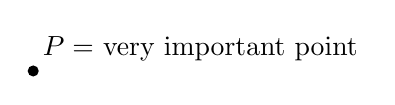
\begin{tikzpicture}
  \fill (0,0) circle (2pt) node[above right] {$P=$ very important point};
\end{tikzpicture}
\end{center}       

How would you describe the location of $P$?  Whether you reference the edges of the page or introduce your own set of axes, you will find that (1) a fixed reference system is required to describe the location, and (2) the resulting description may differ from someone else’s, since different choices of coordinate system lead to different representations.

\begin{idea}
A mathematical object is distinct from its representation.  A single object may have a multitude of representations that depend on convention and convenience.
\end{idea}

\subsection*{How to Create a Coordinate System}

When you first encountered vectors in your earlier courses it was probably assumed that these vectors exist in some established rectangular coordinate system.  Such a coordinate system implicitly postulates the following structure:
\begin{itemize}
    \item Location of the origin
    \item Unit of length
    \item Orthogonality of axes
\end{itemize}

Representation of points and vectors was dictated by the established coordinate system.

What if we started from scratch?  Take two vectors, choose the location of the origin, then use the two vectors to create a coordinate grid.  The interactive below allows you to move points $A$ and $B$ to create two vectors.  Move the slider to see how different points in the plane can be represented using this coordinate grid, and how the representation of a fixed point changes depending on what grid is chosen.

% https://www.geogebra.org/classic/edcyushm
\begin{center}
    \geogebra{edcyushm}{800}{600}
\end{center}

When using an alternative coordinate system, it is customary to identify the vectors that determine it.  For now, we will say that the coordinates of point $P$ are stated with respect to $\{\overrightarrow{OA}, \overrightarrow{OB}\}$.  We will refine this statement later in the text.

\begin{exploration}\label{exp:coordSystemLinCombs1}
Use the interactive below to answer questions about the coordinates of points with respect to various coordinate systems.
% https://www.geogebra.org/classic/qw5dpmqq
\begin{center}
    \geogebra{qw5dpmqq}{800}{600}
\end{center}
\begin{question}
    List the coordinates for each $P_i$ with respect to the given coordinate system.  Your coordinates should be of the form $(\overrightarrow{OA}\text{-coordinate}, \overrightarrow{OB}\text{-coordinate})$.
    $$P_1=\left(\answer{1},\answer{1}\right)$$
    $$P_2=\left(\answer{-2},\answer{0}\right)$$
    $$P_3=\left(\answer{0},\answer{-1}\right)$$
    $$P_4=\left(\answer{-2},\answer{3}\right)$$
    $$P_5=\left(\answer{3},\answer{-2}\right)$$
\end{question}

\begin{question}
REFRESH your browser to return to the original coordinate system.  Move point $A$ to coincide with $P_1$
    List the coordinates for each $P_i$ with respect to the new coordinate system.  
    $$P_1=\left(\answer{1},\answer{0}\right)$$
    $$P_2=\left(\answer{-2},\answer{2}\right)$$
    $$P_3=\left(\answer{0},\answer{-1}\right)$$
    $$P_4=\left(\answer{-2},\answer{5}\right)$$
    $$P_5=\left(\answer{3},\answer{-5}\right)$$
    How do these coordinates compare to the coordinates in the original coordinate system?  Explain why this is happening. (Hint: REFRESH your browser to return to the original coordinate system to compare.)
\end{question}

\begin{question}
REFRESH your browser to return to the original coordinate system. Move point $B$ to coincide with $P_3$
    List the coordinates for each $P_i$ with respect to the new coordinate system.  
    $$P_1=\left(\answer{1},\answer{-1}\right)$$
    $$P_2=\left(\answer{-2},\answer{0}\right)$$
    $$P_3=\left(\answer{0},\answer{1}\right)$$
    $$P_4=\left(\answer{-2},\answer{-3}\right)$$
    $$P_5=\left(\answer{3},\answer{2}\right)$$
    How do these coordinates compare to the coordinates in the previous question?  Explain why this is happening. (Hint: REFRESH your browser to return to the original coordinate system to compare.)
\end{question}

% \begin{question}
%     REFRESH your browser to return to the original coordinate system.  Express each $\overrightarrow{OP}_i$ as a linear combination of $\overrightarrow{OA}$ and $\overrightarrow{OB}$.
% $$\overrightarrow{OP}_1=\answer{1}\overrightarrow{OA}+\answer{1}\overrightarrow{OB}$$
% $$\overrightarrow{OP}_2=\answer{-2}\overrightarrow{OA}+\answer{0}\overrightarrow{OB}$$
% $$\overrightarrow{OP}_3=\answer{0}\overrightarrow{OA}+\answer{-1}\overrightarrow{OB}$$
% $$\overrightarrow{OP}_4=\answer{-2}\overrightarrow{OA}+\answer{3}\overrightarrow{OB}$$
% $$\overrightarrow{OP}_5=\answer{3}\overrightarrow{OA}+\answer{-2}\overrightarrow{OB}$$

% Discuss the relationship between your answers to the first question and your answers here.
% \end{question}

\begin{question}
    Move point $B$ to coincide with $P_2$.  What do you observe?  Do vectors $\overrightarrow{OA}$ and $\overrightarrow{OB}$ determine a good coordinate system for the plane?  Can we express every point in the plane with respect to the coordinate system determined by $\{\overrightarrow{OA}, \overrightarrow{OB}\}$?  Can we express \textit{some} points in the plane with respect to the coordinate system determined by $\{\overrightarrow{OA}, \overrightarrow{OB}\}$?
\end{question}

\end{exploration}

\begin{exploration}\label{exp:coordSystemLinCombs2}
We will use the same set-up as in the previous exploration but introduce an additional vector $\overrightarrow{OC}$.

 % https://www.geogebra.org/classic/b3k96x2w

 \begin{center}
     \geogebra{b3k96x2w}{800}{600}
 \end{center}

 \begin{question}
     Suppose we want to express $P_1$ using a ``coordinate system" determined by three vectors $\overrightarrow{OA}$, $\overrightarrow{OB}$, and $\overrightarrow{OC}$.  Fill in the missing coordinates for $P_1$ below, if the coordinates are to be of the form $(\overrightarrow{OA}\text{-coordinate}, \overrightarrow{OB}\text{-coordinate}, \overrightarrow{OC}\text{-coordinate})$.
     $$P_1=\left(\answer{1},\answer{1},0\right)$$
     $$P_1=\left(0,\answer{2},\answer{0.5}\right)$$
     $$P_1=\left(\answer{2}, 0, \answer{-0.5}\right)$$
     $$P_1=\left(\answer{3},-1,-1\right)$$

How many ways are there to express $P_1$ using this ``coordinate system"?
\begin{multipleChoice}
    \choice{1}
    \choice{4}
    \choice{Infinitely many}
\end{multipleChoice}
 \end{question}

 % \begin{question}
 %     Based on your work above, express $\overrightarrow{OP_1}$ as a linear combination of $\overrightarrow{OA}$, $\overrightarrow{OB}$, and $\overrightarrow{OC}$.  How many ways do you think there are to do this?
 % \end{question}

 \begin{question}
     Compare and contrast the coordinate systems in this exploration and Exploration \ref{exp:coordSystemLinCombs1}.  
 \end{question}
    
\end{exploration}

What we discovered is that not all collections of vectors are adequate for making a useful coordinate system. In Exploration \ref{exp:coordSystemLinCombs1} we learned that if two vectors are collinear, then not all points in the plane can be represented with respect to those two vectors.  In Exploration \ref{exp:coordSystemLinCombs2} we found that having too many vectors results in a point having infinitely many representations, which would be computationally confusing.  

\begin{idea}
    What makes a good coordinate system?
    \begin{itemize}
        \item Every point has coordinates associated with it;
        \item The set of coordinates associated with each point is unique.
    \end{itemize}
\end{idea}


\end{document}